\graphicspath{{chapters/oscillations/images/}}
\chapter{Neutrino Oscillations}
\label{chapter:oscillations}
The search for oscillation events requires an explanation of neutrino oscillations.
Experimental evidence for the neutrino oscillations and current constraints on the oscillation parameters is presented in Sections~\ref{chapter:oscillations}, \ref{sec:superk_atmo}, and \ref{subsec:global_fits}.
The theory of neutrino oscillations is included here with broad descriptions of oscillations in vacuum (Section~\ref{subsec:vacuum}) and in matter (Section~\ref{subsec:msw}). 
Finally, a description of unitarity in the Pontecorvo–Maki–Nakagawa–Sakata (\emph{PMNS}) mixing matrix is given in Section~\ref{sec:unitarity} with particular emphasis placed on the search for additional neutrino flavors (Section~\ref{subsec:steriles}).
The motivation for this thesis as well as the purpose behind joint fits between appearance and disappearance data is discussed in Section~\ref{subsec:steriles_unitarity}.

\section{Solar Neutrinos: A Hint of Multiple Flavors}
\label{bsec:solar_neutrinos}
Early searches for neutrinos focused primarily on the Sun.
The first major experiment, proposed by Ray Davis and John Bahcall, was designed to verify that fusion was the primary energy source of the Sun \cite{Homestake-Bahcall, Homestake-Davis}.
While the core of the sun is not directly visible to conventional telescopes, neutrinos produced via nuclear fusion could escape the sun relatively unchanged and be observed at Earth.

The Homestake experiment, named for Homestake mine in South Dakota, used 615 tons of perchloroethylene to measure neutrinos via the inverse beta decay reaction

\begin{equation}
\nu_e + ^{37}Cl \rightarrow ^{37}Ar + e^- .
\end{equation}

The production rate was well-measured, with a rate of 0.48 counts per day and a background of 0.09 counts per day due to interactions from cosmic ray induced muons \cite{Description-Homestake}.
In the typical units of the solar neutrino experiments, this worked out to 

\begin{equation}
\left(\sigma \phi\right) = 2.56 \pm 0.16 \pm 0.16 \ SNU
\end{equation}
%
where the solar neutrino unit, SNU, is equal to  $10^{-36}$ captures/nucleus/second. 
The expected rate of neutrino interactions from the sun, however, was prediced to be $8.00 \pm 0.97$ SNU given the solar models at the time.
The Homestake experiment, therefore, was only observing approximately 30\% of the prediced interaction rate.
New measurements from other experiments, such has SAGE \cite{Description-SAGE}, GALLEX \cite{Description-GALLEX}, and GNO \cite{Description-GNO} confirmed the results, although with a reduction of around 50\% instead of 70\% compared to theoretical expectations.

The disagreement between the number of neutrinos expected and the number predicted was not definitively solved until the Sudbury Neutrino Observatory (SNO) experiment came online.
SNO was a detector located 2 km underground in the Sudbury mine in Canada \cite{Description-SNO}.
The detector consisted of a large tank filled with heavy water surrounded by photo-multiplier tubes for the detection of Cherenkov emission.
By introducing heavy water, SNO was sensitive to not only the charged current interactions of previous experiments, but also to neutral current interactions invisible to the inverse beta decay experiments.

SNO detected the neutral current and charged current interactions via two distinct channels. 
The charged-current interactions caused a deuterium atom to break down into two separate protons while also transforming the neutrino into an electron.
The electron would be produced with an energy high enough to emit Cherenkov radiation and could, therefore, be observed directly, with the energy of the electron used to constrain the incident neutrino spectrum.
The primary charged current interaction at SNO was only sensitive to electron flavor neutrino interactions.

The neural current interactions, with a threshold energy of 2.22 MeV, were able to separate the deuterium in the heavy water, leading to a free neutron in the detector. 
The detection of the free neutron posed initial challenges for the same fundamental reason that neutrino detection is difficult: neutrons are not charged and therefore do not emit electromagnetic radiation.
Instead, early detections of these neutrons relied on the emission of a high energy gamma ray when the neutron was captured on a deuterium atom.
The gamma ray could then, in turn, be absorbed on an electron, accerating the charged particle and producing Cherenkov radiation.

Measurements at SNO were divided between these two channels in order to investigate one possible solution to the missing solar neutrinos: neutrino oscillations \cite{SNO-Proposal}.
Because the three known neutrino states all have the same neutral current interaction cross section, the neutral current rate is expected to be constant in the presence of oscillations.
The charged current rate is, however, expected to change due to the different couplings of each neutrino flavor to the $W^{\pm}$ boson.
Measuring both the neutral current and charged current rates therefore provided a direct test of neutrino oscillations, allowing researchers to identify the effect independent of the solar model.

SNO expected a rate of neutral current interactions from solar neutrinos of $5.05 \times 10^6 cm^{-2} s^{-1}$ and an equivalent observed 

\begin{equation}
\phi_{NC}\left(\nu \ active \right) = 5.25 \pm 0.16 (stat) ^{+0.11}_{-0.13} \times 10^6 cm^{-2} s^{-1}
\end{equation}
%
a result consistent with expectations.
The charged current interaction was measured to be only 30\% of the expected rate, clearly indicating that the number of electron neutrinos was well below expectations.
The combination of these two results gave the first clear indication of neutrino oscillations, a result which earned the director of the experiment, Art McDonald, a Nobel Prize in 2015 \cite{NobelPrize:2015-Oscillations}.

\section{Super-Kamiokande and Atmospheric Neutrinos}
\label{sec:superk_atmo}
While the SNO experiment was working to identify the source of the solar neutrino deficit, the Kamioka Nucleon Decay Experiment (KamiokaNDE) and its successor, Super-Kamiokande (Super-K), were using a similar water Cherenkov detector to search for proton decay.
The primary background for this rare process is neutrino interactions.
Unlike SNO, however, Super-Kamiokande was sensitive to both MeV solar neutrinos and GeV neutrinos produced in the atmospheric showers from cosmic ray interactions. 

\begin{figure}[h]
\centering
\begin{tabular}[b]{c}
  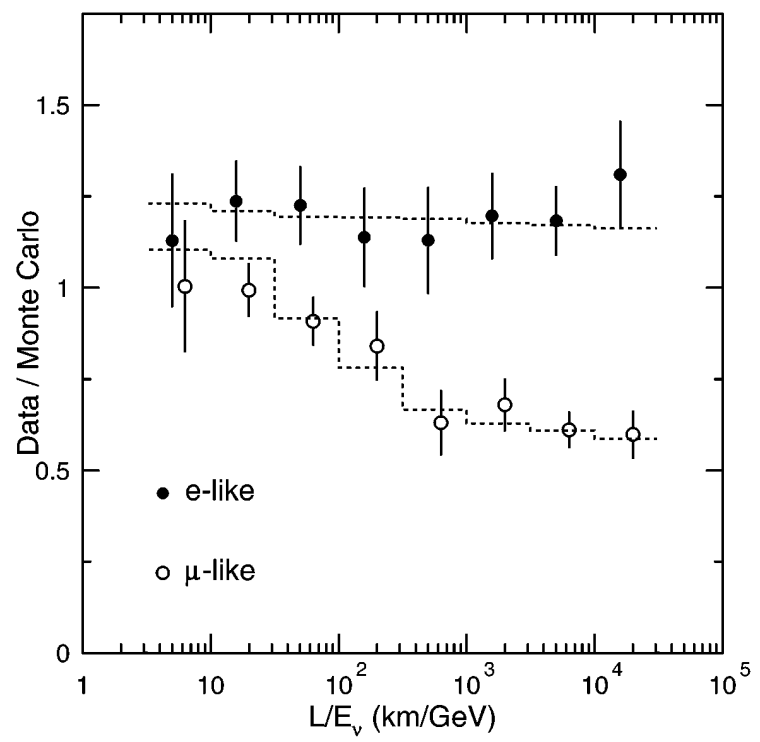
\includegraphics[width=0.45\linewidth]{superk_l_over_e.png} \\
  \small (\textbf{\color{ctcolormain}a}) L/E From \cite{SuperK-Oscillations}
\end{tabular} \hspace{2pt}
\begin{tabular}[b]{c}
  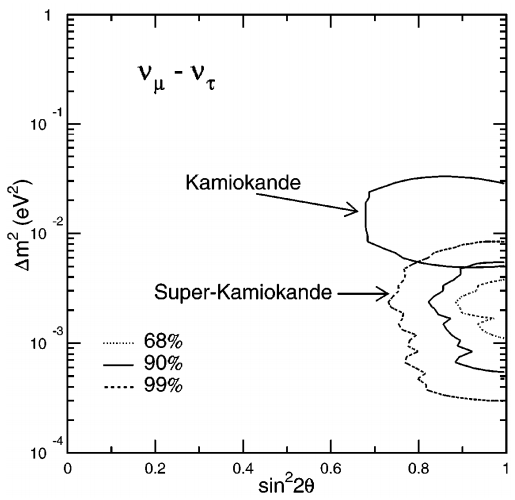
\includegraphics[width=0.45\linewidth]{superk_discovery.png} \\
  \small (\textbf{\color{ctcolormain}b}) Oscillation Measurement from \cite{SuperK-Oscillations}
\end{tabular}
	\caption[The first atmospheric oscillation results from Super-Kamiokande}{The first atmospheric neutrino oscillation measurements from the Super-K experiment. (a) The $\nu_e$-like events show no shape in L/E, as expected from a lack electron neutrino oscillations at these L/E scales. The $\nu_\mu$-like interactions, however, show a clear drop, indicating the presence of oscillation effects. (b) Using the two neutrino approximation, Super-K produced contours of the best-fit oscillation parameters for $\nu_\mu\rightarrow\nu_\tau$ oscillations. Both figures from \cite{SuperK-Oscillations}}
	\label{fig:superk_atmo}
\end{figure}


While investigating backgrounds, Super-Kamiokande observed an interesting deficit in the atmospheric neutrino signal.
Unlike the case in the solar neutrinos, the deficit observed by Super-K was observed solely in the muon neutrino events with no effect seem in the electron neutrinos \cite{SuperK-Oscillations}.
Using the reconstructed energy and direction of events, Super-K was able to show that the number of fully contained events of $\nu_\mu$-like interactions changed as a function of L/E - a clear signature of neutrino oscillations in the atmospheric neutrinos.
The figure, reproduced in Figure~\ref{fig:superk_atmo}, was used, in part, with an 2x2 approximation to the PMNS matrix to produce the first measurements, shown in Figure~\ref{fig:superk_atmo}, of the atmospheric oscillation parameters.
For the discovery of atmospheric neutrino oscillations at the same time as SNO's discovery of solar neutrino oscillations, Takaaki Kajita was awarded the 2015 Nobel Prize \cite{NobelPrize:2015-Oscillations}.




\section{Oscillation Theory and the PMNS Matrix}
\label{sec:oscillation_theory}
In 1968, Bruno Pontecorvo suggested a process, known as \emph{neutrino oscillation}, by which neutrinos could change flavors \cite{Pontecorvo-Oscillations}.
The theory of neutrino oscillations was further developed for the neutrino sector by Ziro Maki, Masami Nakagawa and Shoichi Sakata in 1962 \cite{Maki-Nakagawa-Sakata}.

\subsection{The PMNS Mixing Matrix}
We now understand there to be three distinct flavors of neutrinos.
Neutrinos interact via the weak force and are created in flavor eigenstates ($\nu_e , \nu_\mu , \nu_\tau$) describing the fields of the left-handed neutrinos.
These flavor states couple via the weak charge to the electron, muon, and tau respectively.

The three weak eigenstates are related to three known neutrino mass eigenstates, $\nu_1$, $\nu_2$, and $\nu_3$, via the Pontecorvo-Maki-Nakagawa-Sakata (\emph{PMNS}) lepton mixing matrix.

\begin{equation}
\begin{pmatrix} \nu_e \\ 	\nu_\mu \\	\nu_\tau \end{pmatrix} = 
U_{PMNS} \begin{pmatrix} \nu_e1\\ 	\nu_2 \\	\nu_3 \end{pmatrix} = 
\begin{pmatrix}
 U_{e 1} & U_{e 2} & U_{e 3} \\
 U_{\mu 1} & U_{\mu 2} & U_{\mu 3} \\
 U_{\tau 1} & U_{\tau 2} & U_{\tau 3} \\
\end{pmatrix} 	
\begin{pmatrix} \nu_1 \\ 	\nu_2 \\	\nu_3 \end{pmatrix}
\label{eqn:3flavor_pmns}
\end{equation}

This may be written in the shortened form

\begin{equation}
\nu_{\alpha}\left(x\right) = \sum_i U_{\alpha i} \nu_{i}\left(x\right)
\label{eqn:3flavor_short}
\end{equation}
%
where ${\alpha=e,\mu,\tau}$ and ${i=1,2,3}$. 

As a 3 ${\times}$ 3 unitary matrix, the PMNS matrix may be parametrized in terms of three mixing angles and six phases.
Of these phases, five may be removed by rephasing the lepton fields with no change to the underlying physics, leaving one physical phase ralted to CP violation.

The PMNS matrix may be written in terms of the product of three smaller unitary matrices, each described by a \emph{mixing angle} $\theta_{ij}$: 

\begin{equation}
U_{PMNS} = 
\begin{pmatrix}
1 & 0 & 0 \\
0 & c_{23} & s_{23} \\
0 & -s_{23} & c_{23} \\
\end{pmatrix}
\begin{pmatrix}
c_{13} & 0 & s_{13} e^{-i\delta_{CP}} \\
0 & 1 & 0 \\
-s_{13} e^{i \delta_{CP}} & 0 & c_{13} \\
\end{pmatrix}
\begin{pmatrix}
c_{12} & s_{12} & 0 \\
-s_{12} & c_{12} & 0 \\
0 & 0 & 1 \\
\end{pmatrix}
\label{eqn:pmns_parametrized}
\end{equation}
%
where ${c_{ij}}$ denotes ${\cos\left(\theta_{ij}\right)}$ and ${s_{ij}}$ denotes ${\sin\left(\theta_{ij}\right)}$.

Note that if neutrinos are Majorana fermions, the additional phases may not be removed without making the masses complex.
The Majorana terms form additional diagonal terms in Equation~\ref{eqn:pmns_parametrized}.
While Majorana mass terms are beyond the scope of this work, further information may be found in \cite{Review-PMNS,Review-MajoranaNu}.

The three submatrices of Equation~\ref{eqn:pmns_parametrized} have historically been studied by different types of experiments. 
This history has lead to the proliferation of alternative names for the matrices and of the mixing angles.

\begin{equation}
U_{PMNS} = U_{Atmospheric} U_{Reactor} U_{Solar}
\end{equation}
%
This leads to the alternative names of the mixing angles, with ${\theta_{23}}$, ${\theta_{13}}$, and ${\theta_{12}}$ being referred to as the atmospheric mixing angle, the reactor mixing angle, and the solar mixing angle respectively.

\subsection{Neutrino Mixing in Vacuum}
\label{subsec:vacuum}
Neutrinos are created in pure flavor eigenstates.
To propagate the neutrino, the Hamiltonian must be applied to the state.
The flavor eigenstate of the initial neutrino is not an eigenstate of the Hamiltonian, however.
Instead, the neutrino state must be written in terms of the mass eigenstates

\begin{equation}
\ket{\nu\left(t=0\right)} = \ket{\nu_\alpha} = \sum_i U_{\alpha i} \ket{\nu_i}.
\end{equation}

After propagation for a time $t \neq 0$, the state will no longer be a pure flavor state.

\begin{equation}
\ket{\nu\left(t\right)} = \sum_i U_{\alpha i} e^{-iE_i t} \ket{\nu_i}
\end{equation}

where ${E_i} = \sqrt{p^2+m_i^2}$ is the total energy of the ${i}$th mass eigenstate.
If the neutrino interacts, the flavor eigenstate must again be used to calculate the probabilities of interacting as each of the three known flavors.

\begin{equation}
P\left(\nu_\alpha\rightarrow\nu_\beta\right) = \left|\bra{\nu_\beta}\ket{\nu_\alpha\left(t\right)}\right|^2 
                 															= \left|\sum_i U_{\beta i} U^*_{\alpha i} e^{-i E_i t} \right|^2
\label{eqn:pmns_probability}
\end{equation}

Proper calculations from this point can be performed by treating each neturino as a quantum mechanical wave packet \cite{OscillationWavePackets}.
This allows for the full description of neutrino oscillation in the context of decoherence of the mass states during propagation, allowing each mass state to possess separate momenta.

In practice, the description of neutrino oscillations necessary for this work is adequately described by making a few simplifying assumptions.
In particular, this work assumes that all mass eigenstates propagate as plane waves possessing identical, well-defined momenta \cite{Review-PMNS}.
Neutrinos are further assumed to be extremely relativistic at the energies of interest, an assumption well-justified by cosmological fits to the sum of the three neutrino masses, which give an upper limit of around 0.2 eV \cite{PDG-2015}.
The total neutrino energy is also assumed to be unchanged during propagation.
The resulting calculation of the oscillation probabilities is identical in both the simplified version and the full derivation.

To begin, equation~\ref{eqn:pmns_probability} is expanded by explicitly including the complex conjugate,  
\begin{equation}
P\left(\nu_\alpha\rightarrow\nu_\beta\right) =  \sum_i^3 U^*_{\beta i} U_{\alpha i} \sum_j^3 U_{\beta j} U^*_{\alpha j} e^{i \left(E_i-E_j\right) t} \ \ \ \alpha,\beta = e,\mu,\tau.
\label{eqn:pmns_probability_expanded}
\end{equation}

In the highly relativistic limit, $E \gg m_{i}$, and $t \approx L$ where $L$ is the distance traveled during propation.
Using these two approximations, the exponential term in Equation~\ref{eqn:pmns_probability} may be rewritten using Euler's formula as

\begin{equation}
 e^{i \left(E_i-E_j\right) t} = 1 - 2\sin^2\left(\frac{\Delta m_{ij}^2 L}{4E}\right) + i \sin\left(\frac{\Delta m_{ji}^2 L}{2E}\right)
\end{equation}
%
where $\delta_{\alpha \beta}$ is the Kronecker delta function.
Note that a new shorthand has been defined, ${\Delta m^2_{ji} = m^2_j - m^2_i}$, giving a fundamental parameter of neutrino oscillations.
The PMNS terms of equation~\ref{eqn:pmns_probability_expanded} may be expanded further, yielding 

\begin{equation}
\left| \sum_j U_{\beta j} U^*_{\alpha j}\right|^2 = \delta_{\alpha \beta} + 2 \sum_{i<j} \sum_i U^*_{\beta i} U_{\alpha i}  U_{\beta j} U^*_{\alpha j}
\end{equation}
%
where the factor of two arises due to the symmetry ${i \leftrightarrow j}$.
Putting the terms together, the final oscillation probability formula is

\begin{equation}
\begin{aligned}
P\left(\nu_\alpha\rightarrow\nu_\beta\right) ={} &	 \delta_{\alpha \beta} -  4 \sum_{i<j} Re\left[ \sum_i U^*_{\beta i} U_{\alpha i}  U_{\beta j} U^*_{\alpha j} \right] \sin^2\left(\frac{\Delta m_{ij}^2 L}{4E}\right) \\
	& + 2 \sum_{i<j} Im\left[ \sum_i U^*_{\beta i} U_{\alpha i}  U_{\beta j} U^*_{\alpha j} \right] sin\left(\frac{\Delta m_{ji}^2 L}{2E}\right).
\end{aligned}
\label{eqn:oscil_probabilities}
\end{equation}

The PMNS matrix terms may be replaced in terms of the mixing angles using Equation~\ref{eqn:pmns_parametrized}.

This calculation has been derived for neutrinos.
To calculate the probabilities for anti-neutrinos, the calculation changes by replacing ${U \rightarrow U^*}$, resulting in a change in sign of the last term of Equation~\ref{eqn:oscil_probabilities}.

From Equation~\ref{eqn:oscil_probabilities}, the general form of the oscillation probabilities becomes clear. 
The PMNS matrix elements yield the amplitude of oscillations, while the frequency of the oscillations is related to three quantities: the squared difference in the masses, ${\Delta m^2_{ji}}$; the baseline, or distance traveled, ${L}$; and the energy of the neutrinos.
Only one of these three is a fundamental physics parameter.
The choices of energy and baseline are used to define characteristics of detectors used for measurements of the various mass splitting parameters and oscillation mixing angles.

Note that the oscillation probability is insensitive to the sign of the mass splitting parameter.

\subsection{Matter Effects in Oscillation}
\label{subsec:msw}
Calculations up to this point have assumed neutrinos oscillating in vacuum.
Modifications required for a description of matter effects begin with a modification of the Hamiltonian with a potential, ${V}$, due to coherent forward scattering of neutrino on electrons and nucleons in the medium \cite{Review-MSW}.

\begin{equation}
H = H_0 + V
\end{equation}

The value of ${H_0}$ is the value of vacuum Hamiltonian.
In the two-flavor case, the Hamiltonian can be shown \cite{Review-PMNS,Review-PMNS2} to be

\begin{equation}
H_0 = \frac{\Delta m^2}{4E}
\begin{pmatrix}
- 2 \cos 2 \theta & \sin 2 \theta \\
\sin 2 \theta & 0 \\
\end{pmatrix}.
\end{equation}
%
where ${\theta}$ is the mixing angle associated with the 2x2 PMNS matrix.
The potential includes contributions from both charged current and neutral current interactions, although the charged current interactions arise solely from the electron neutrinos.
The potential, expressed in the flavor basis, is then

\begin{equation}
V_{CC,\alpha} = 
\begin{cases}
\sqrt{2} \pm G_F n_e \left( x\right) & \alpha = e \\
0 & \alpha = \mu, \tau
\end{cases}\ \ \ \ \ 
V_{NC,\alpha} = -\frac{G_F}{\sqrt{2}} n_e\left(x\right)\;\;\; \alpha = e, \mu, \tau
\end{equation}
%
where a + is used for neutrinos and a - is used for antineutrinos, ${n_e}$ is the density of electrons in the medium, and ${G_F}$ is the Fermi coupling constant.
Note that the angle included here is that of the PMNS matrix in two dimensions.
A full description of three flavor neutrino oscillation in the presence of a matter potential may be found in \cite{Review-PMNS,Review-PMNS2}.
The full three-flavor oscillation calculation is used for this thesis using the Prob3++ code \cite{Barger-Oscillations,prob3}, which includes an implementation of matter effects.









\subsection{Global Fits to Oscillations}
\label{subsec:global_fits}
Since the initial discoveries of SNO and Super-K, many experiments have measured neutrino oscillations. 
Global fits are performed and updated regularly \cite{NuFit_2.2, NuFit.org}.

The most recent results are shown in Figure~\ref{fig:nufit_v32} and include information from solar, reactor, and atmospheric oscillation experiments.
The results explicitly assume unitarity of the PMNS mixing matrix and three neutrino species.

\begin{figure}[!h]
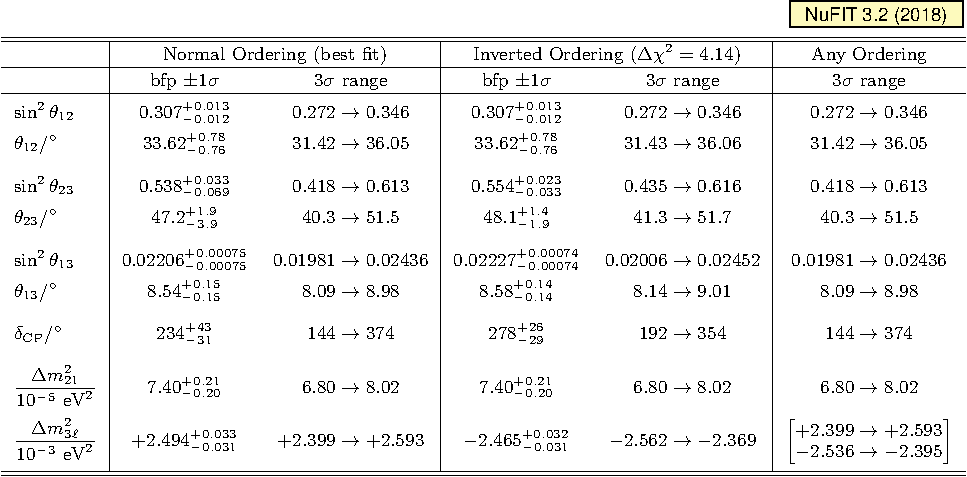
\includegraphics[width=\linewidth]{nufit_v32.pdf}
\caption[Global best fit neutrino oscillation parameters from Nu-Fit.org]{The global best-fit values for the three flavor neutrino oscillation fits as of November 2017. The first column shows results assuming the normal ordering while the second colum shows the results for the inverted ordering. Image taken from \cite{NuFit.org}}
\label{fig:nufit_v32}
\end{figure}

In this thesis, a measurement of atmospheric oscillations at 20 GeV will be performed. 
Plots of the oscillation probabilities using the global fit values of Figure~\ref{fig:nufit_v32} is shown in Figure~\ref{fig:oscil_probs}.




\begin{figure}
\centering
\begin{tabular}{cc}
    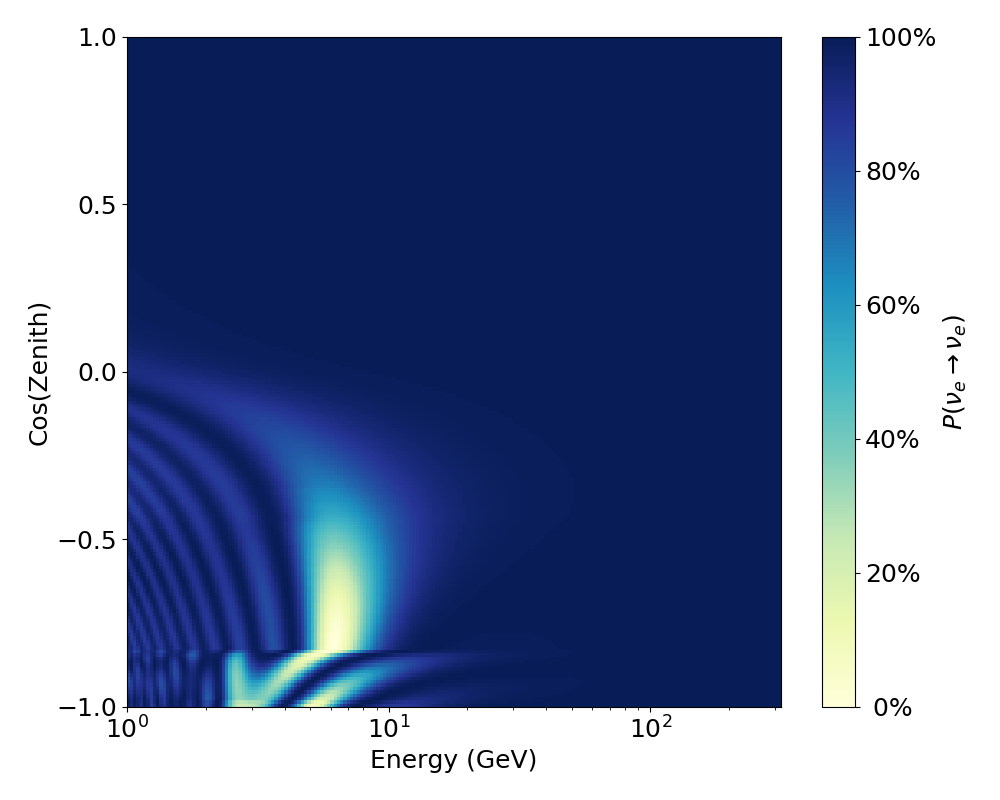
\includegraphics[width=0.48\linewidth]{prob3_nue_nue.png} &  
    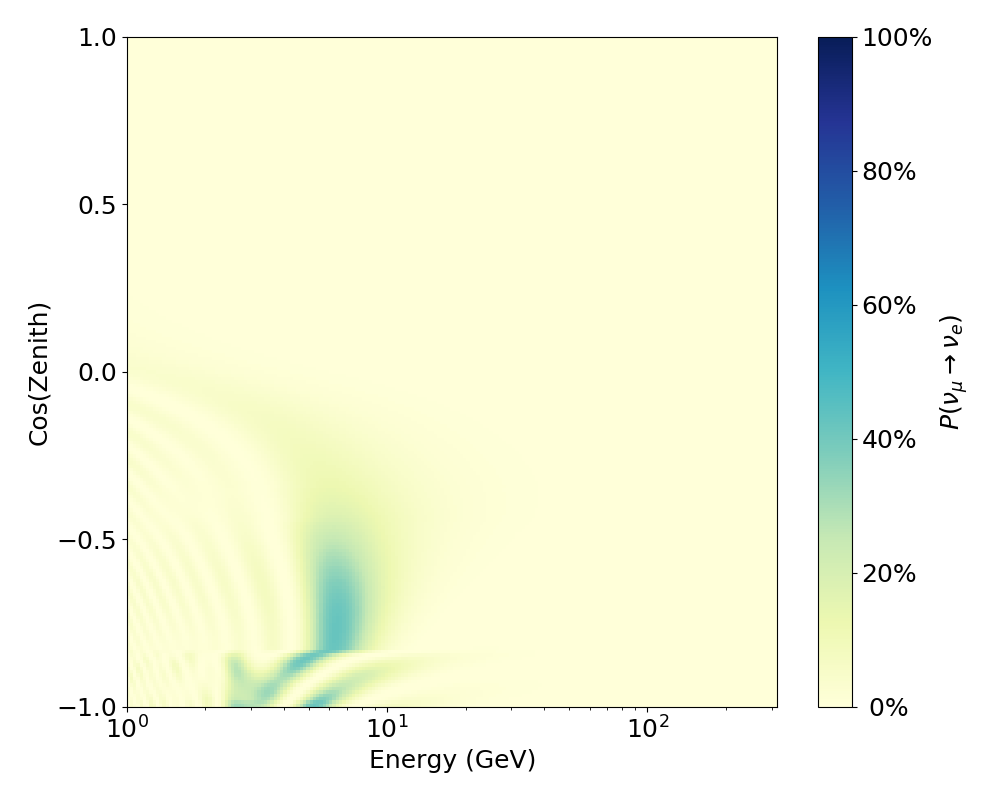
\includegraphics[width=0.48\linewidth]{prob3_numu_nue.png} \\  

    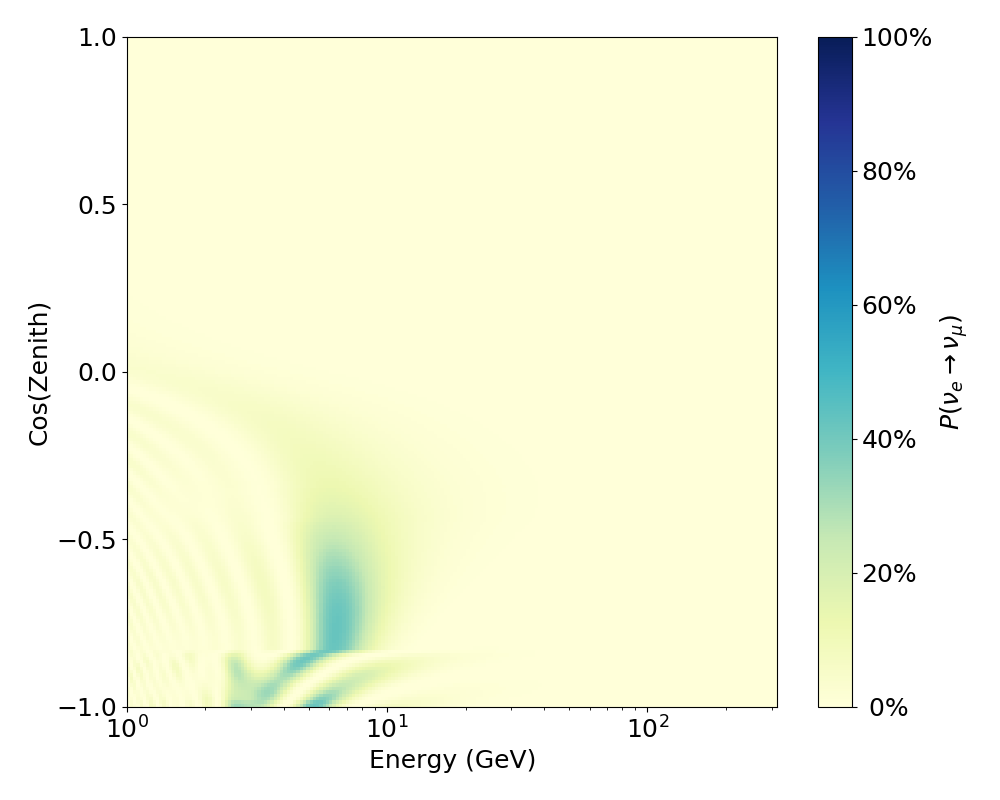
\includegraphics[width=0.48\linewidth]{prob3_nue_numu.png} &  
    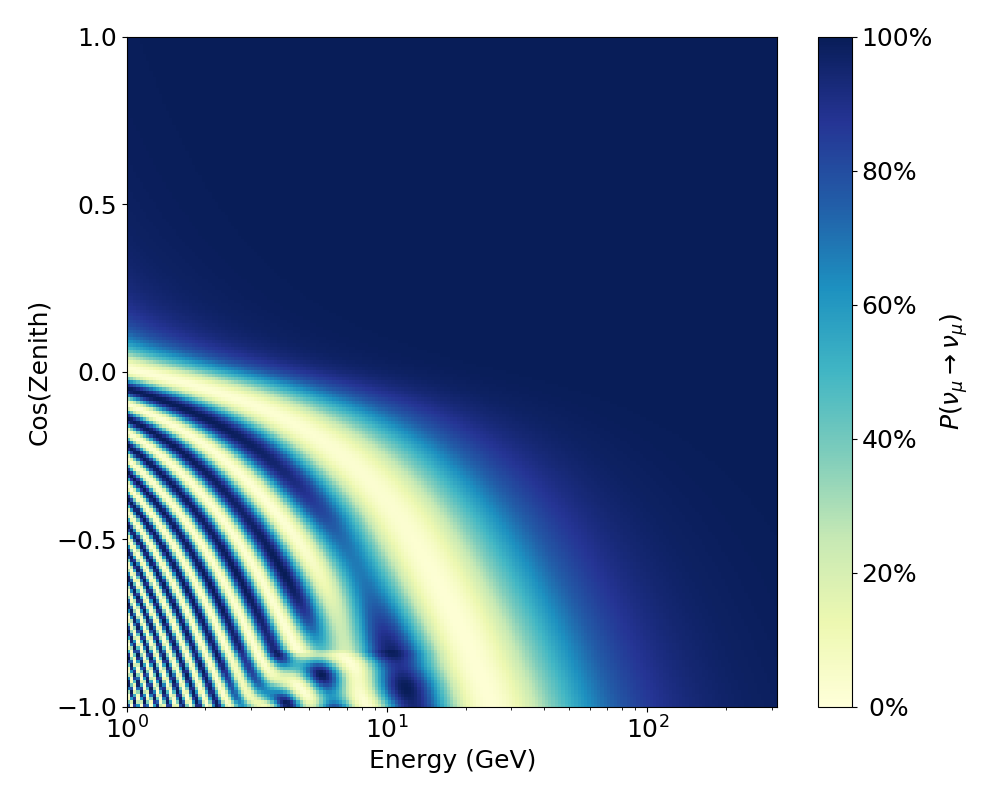
\includegraphics[width=0.48\linewidth]{prob3_numu_numu.png} \\  

    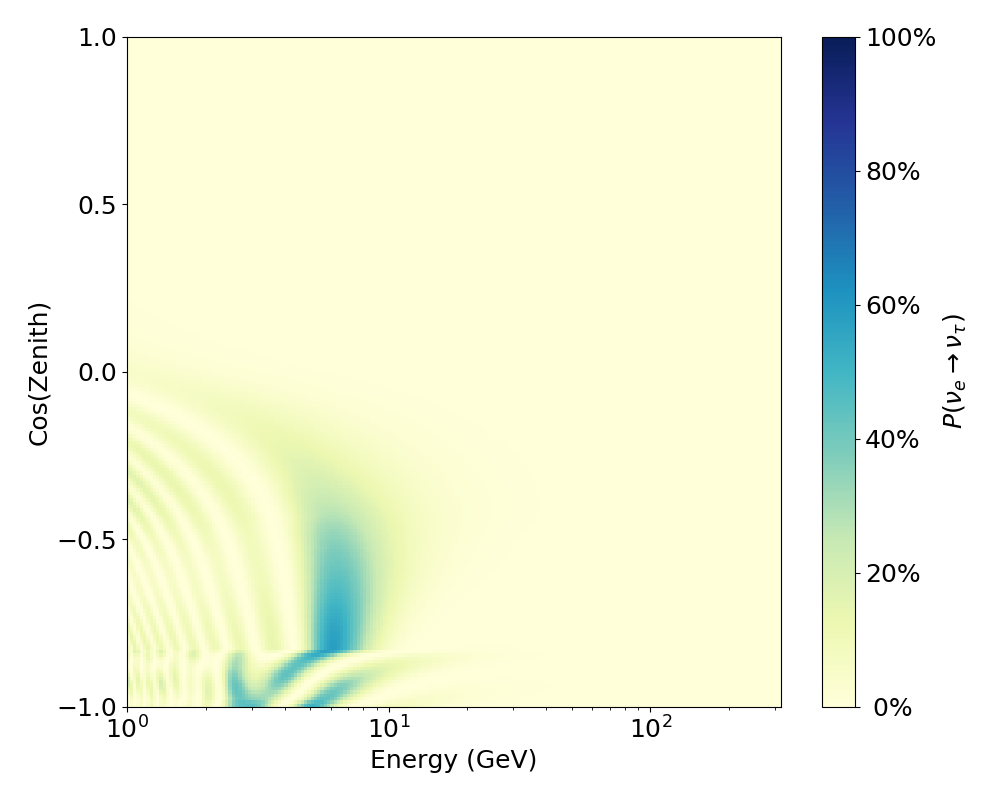
\includegraphics[width=0.48\linewidth]{prob3_nue_nutau.png} &  
    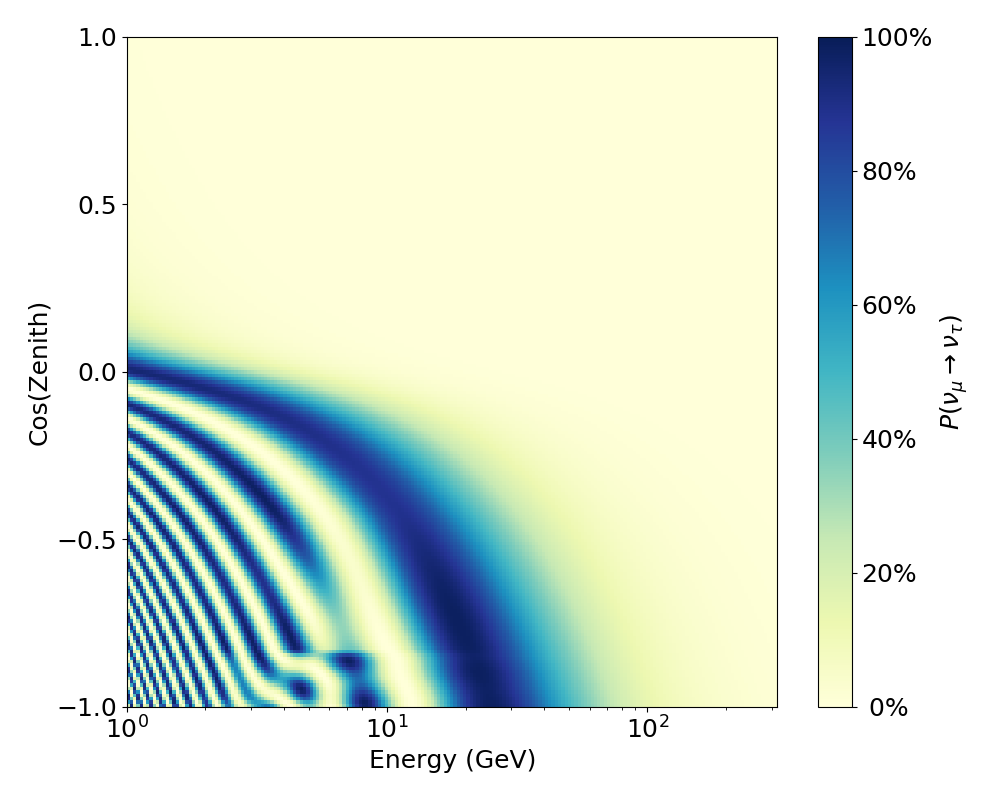
\includegraphics[width=0.48\linewidth]{prob3_numu_nutau.png} \\ 
\end{tabular}
\caption[Oscillation probabilities between 1 and 300 GeV]{The oscillation probabilities for (left) electron neutrinos and (right) muon neutrinos from 1 to 300 GeV. The top row shows the oscillation probabilities to electron neutrinos, the middle row shows the oscillation to muon neutrinos, and the bottom row shows the oscillation to tau neutrinos. }
\label{fig:oscil_probs}
\end{figure}










\section{Unitarity of the Mixing Matrix}
\label{sec:unitarity}
While global fits assume three flavors of neutrinos, additional neutrino flavors are theoretically possible.
The number of active neutrino flavors is limited to the three known flavors from the measurements of the Z boson invisible decay width (see the discussion of Section~\ref{sec:neutrinos}), although such measurements implicitly only measure the number of species with a coupling to the Z boson \cite{ALEPH-3Nu}.
Additional flavors with no or very small couplings to the Z boson are not excluded \cite{Review-LightSterile}.
New neutrino flavors introduced with these properties are known as \emph{sterile neutrinos}.

The effect of sterile neutrinos on the unitarity measurements will be discussed here, although it should be noted that sterile neutrinos aren't the only possible source of non-unitarity.
Any new physics models that include flavor violation, including  non-standard interactions or neutrino decay models can also induce apparent non-unitarity in the 3x3 PMNS mixing matrix.
For the purposes of this thesis, the sterile neutrinos offer a useful insight into one possible cause. 


\subsection{Sterile Neutrinos}
\label{subsec:steriles}
Models of sterile neutrinos assume that no weak interactions are available to the new species.
Instead, sterile neutrinos are assumed to interact with the three active neutrinos via oscillations.
In this model, neutrinos oscillate using a 4x4 (or larger NxN) PMNS matrix \cite{Review-PMNS, GlobalSteriles-2012, GlobalSteriles-2017, Review-LightSterile}.

\begin{equation}
\begin{pmatrix} \nu_e\left(x\right) \\ 	\nu_\mu\left(x\right) \\	\nu_\tau\left(x\right) \\  \nu_s\left(x\right)\end{pmatrix} = 
U_{4\times 4} \begin{pmatrix} \nu_e\left(x\right) \\ 	\nu_\mu\left(x\right) \\	\nu_\tau\left(x\right) \\	\nu_s\left(x\right)\end{pmatrix} = 
\begin{pmatrix}
 U_{e 1} & U_{e 2} & U_{e 3} & U_{e 4} \\
 U_{\mu 1} & U_{\mu 2} & U_{\mu 3} & U_{\tau 4}  \\
 U_{\tau 1} & U_{\tau 2} & U_{\tau 3} & U_{\tau 4}  \\
 U_{s 1} & U_{s 2} & U_{s 3} & U_{s 4}  \\
\end{pmatrix} 	
\begin{pmatrix} \nu_1\left(x\right) \\ 	\nu_2\left(x\right) \\	\nu_3\left(x\right) \\ \nu_4\left(x\right) \end{pmatrix}
\label{eqn:4flavor_pmns}
\end{equation}

The additional terms in $U_{4\times 4}$ lead to new mixing angles, $\theta_{14}$, $\theta_{24}$, and $\theta_{34}$.
The new terms may be used in the standard oscillation framework introduced in Section~\ref{subsec:vacuum} extended with a fourth flavor state, ${\nu_s}$, and mass state, ${\nu_4}$.

\begin{equation}
P\left(\nu_\alpha\rightarrow\nu_\beta\right) =  \sum_i^{4} U^*_{\beta i} U_{\alpha i} \sum_j U_{\beta j} U^*_{\alpha j} e^{i \left(E_i-E_j\right) t} \ \ \ \alpha,\beta = e,\mu\tau,s
\label{eqn:sterile_pmns_probability_expanded}
\end{equation}

Unlike the three active neutrinos, sterile neutrinos cannot interact with matter, leading to a deficit in the neutrino rates from oscillations of the form ${P\left(\nu_\alpha\rightarrow\nu_s\right)}$.
The location and size of the deficit is determined by the oscillation parameters associated with the ${\nu_s}$ and ${\nu_4}$ states.
Sterile neutrinos may be indirectly observed through this deficit by studying the active neutrinos with either charged current or neutral current interactions.
The effects of steriles can also be observed through the MSW and resonance effects for neutrinos that pass through the Earth \cite{IceCubeSterile-IC86-1}.

\subsection{Direct Searches for Steriles}
While oscilation of the three active neutrinos preserves the total neutral current rate, sterile neutrinos do not.
This provides a unique experimental signature for sterile neutrinos.
Dedicated searches for this disappearance have been performed by MINOS \cite{MINOS-SterileNC-2011,MINOS-SterileNC-2016} and NO${\nu}$A \cite{NOvA-SterileNC} with assumptions on the new terms of the mixing matrix.
The effect of three sterile hypotheses on the MINOS data is shown in Figure~\ref{fig:nc_steriles}a. 
Around 15\% of the neutral current events disappear in the three hypotheses tested by MINOS.
The results of the NO${\nu}$A search are shown in Figure~\ref{fig:nc_steriles}b.


\begin{figure}[h]
\centering
\begin{tabular}[b]{c}
  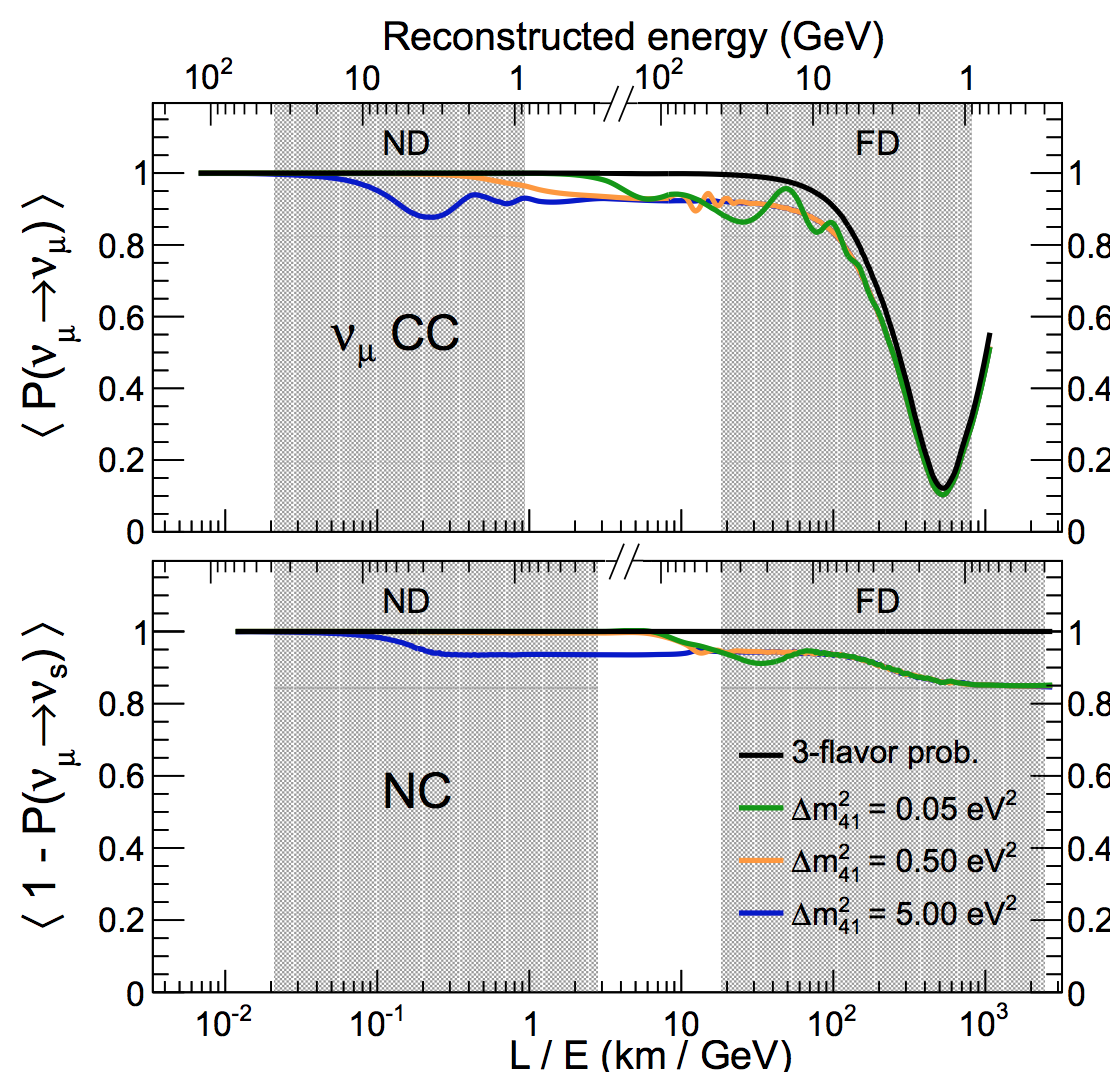
\includegraphics[width=0.45\linewidth]{minos_sterile_nc.png} \\
  \small (\textbf{\color{ctcolormain}a}) MINOS NC Sterile Expectation
\end{tabular} \hspace{2pt}
\begin{tabular}[b]{c}
  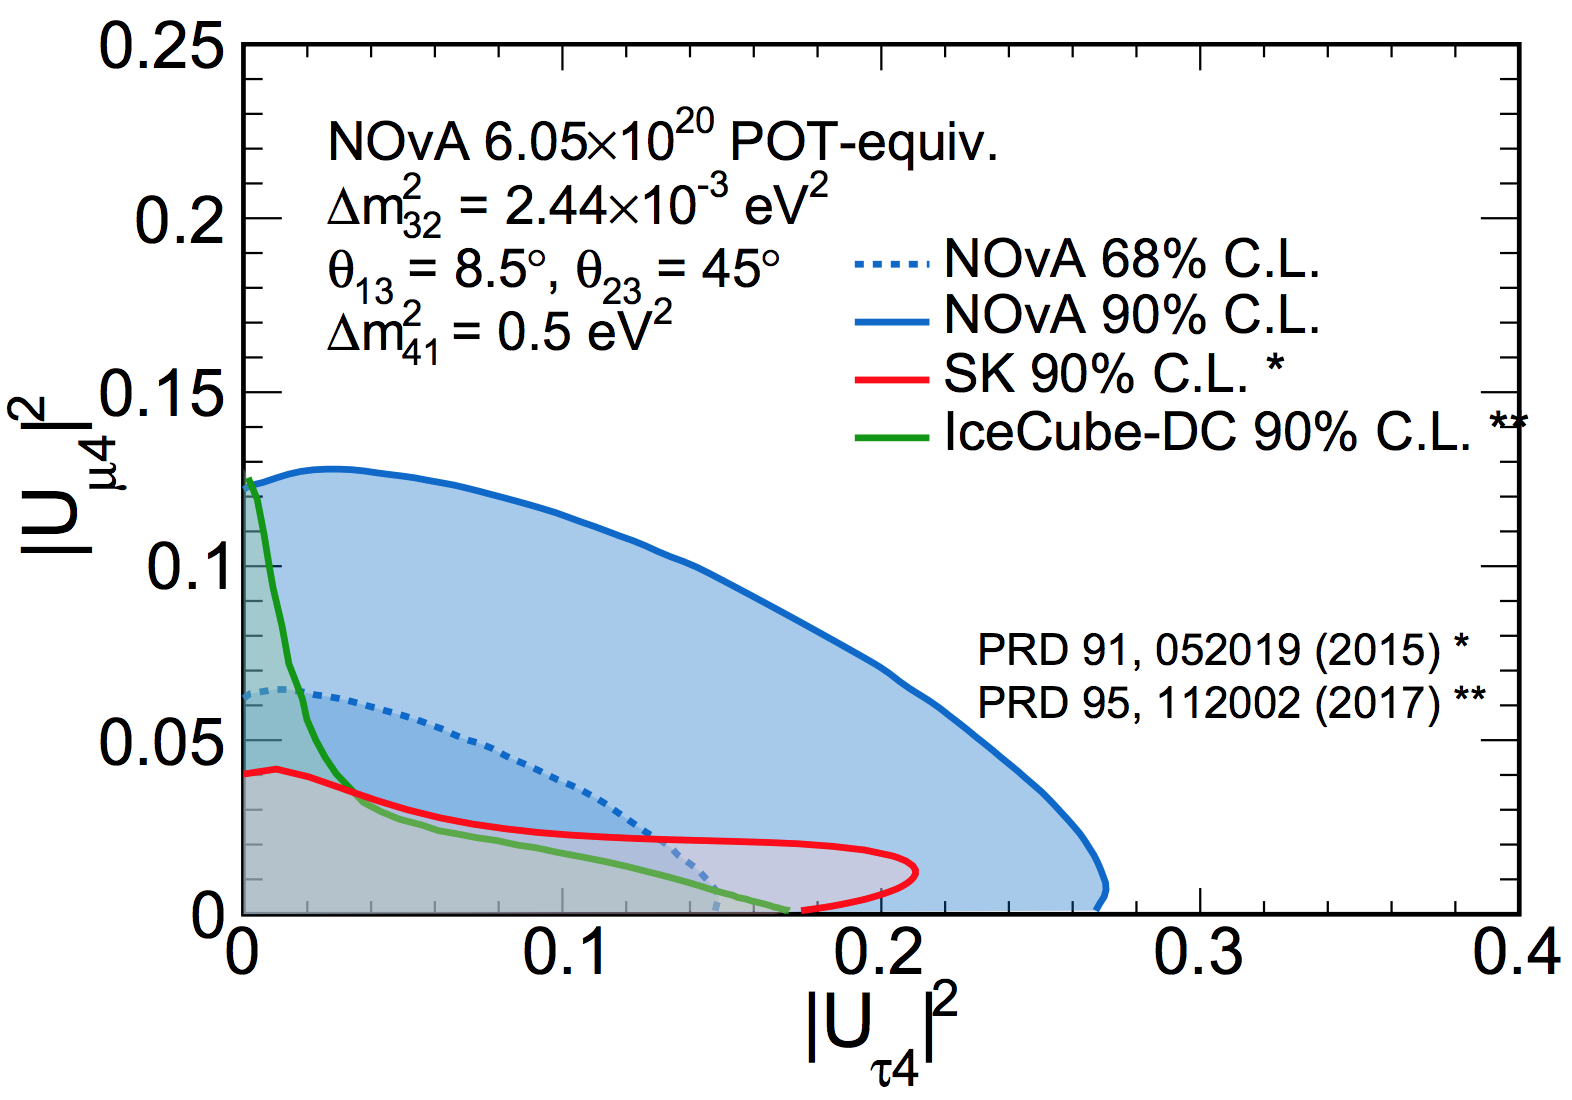
\includegraphics[width=0.45\linewidth]{nova_sterile_constraints.png} \\
  \small (\textbf{\color{ctcolormain}b}) NO${\nu}$A Limits from NC Oscillations
\end{tabular}
\caption[The MINOS and NO$\nu$A NC oscillation search results]{Expectations (a) and results (b) of searches for sterile neutrinos in the neutural current interactions. (a) Effect of three hypothetical sterile neutrinos on the measurements of the MINOS detector \cite{MINOS-SterileNC-2016}. "ND" and "FD" refer to the near and far detector of MINOS respectively. The sterile neutrinos have a small effect on the main oscillation minimum in the charged current channel, but up to 15\% of the neutral current events are lost. (b) The results of the NO${\nu}A$ search for sterile neutrinos using neutral current events. The limits are interpreted in terms of the 4$\times$4 PMNS mixing elements in order to compare to searches with charged current interactions in Super-Kamiokande \cite{SuperK-Steriles2015} and IceCube \cite{IceCubeSterile-Andrii}. }
\label{fig:nc_steriles}
\end{figure}

Most experiments attempt to investigate one of the additional terms only, assuming the remainder to be negligible \cite{SuperK-Steriles2015, IceCubeSterile-Andrii, IceCubeSterile-IC86-1}. 
The results rule out large mixing between a hypothetical sterile neutrino and the three active flavors, although small mixing angles are still allowed by experiments \cite{GlobalSteriles-2017, Review-LightSterile}.

\subsection{Indirect Searches for Steriles Using Unitarity}
\label{subsec:steriles_unitarity}
The addition of a fourth generation of neutrino would have consequences for neutrino oscillation measurements performed in the 3x3 PMNS framework.
Standard 3-flavor oscillation measurements may therefore be used to place limits on sterile neutrinos.

The PMNS matrix gives the change in basis and is assumed to be unitary.
The unitary condition imposes summation rules for both the rows and columns of the matrix \cite{Parke-Unitarity}.

\begin{equation}
\sum_i \left| U_{\alpha i} \right|^2 = 1 \;\;\;\; \alpha=e, \mu, \tau
\label{eqn:unitarity_condition_flavor}
\end{equation}
\begin{equation}
\sum_\alpha \left| U_{\alpha i} \right|^2 = 1 \;\;\;\; i=1,2,3
\label{eqn:unitarity_condition_mass}
\end{equation}

If the neutrino mixing matrix consists of more than the three known active neutrinos, however, these unitary relations would only hold in higher dimensions.
When projected down to the a 3x3 PMNS matrix, non-unitarity would be observed.

Neutrino oscillation measurements are performed with the assumption of 3x3 unitarity imposed, allowing the PMNS matrix to be rewritten in terms of three mixing angles and a single phase.
The appearance and disappearance probabilities in oscillation measurements are typically written in terms of these mixing angles.
Using these mixing angles, the disappearance probability for atmospheric oscillations of $\nu_\mu \rightarrow \nu_\mu$ is given by

\begin{equation}
\begin{aligned}
P\left(\nu_\mu\rightarrow\nu_\mu\right) &{}=  1 -  \left| \sum_i U^*_{\mu i} U_{\mu i} e^{-i m_i^2 L/2E} \right|^2 \\
 						&{}= 1 - \left( \cos^2 \theta_{13} \sin^2 2 \theta_{23} + \sin^4 \theta_{23} \sin^2 2 \theta_{13} \right) \sin^2 \left( \frac{\Delta m^2_{31} L}{4 E} \right) \\
 						&{}\approx 1 - \sin^2 2 \theta_{23} \sin^2 \left(\frac{\Delta m^2_{31} L}{4 E} \right).
\end{aligned}
\label{eqn:mu_disappearance_probability}
\end{equation}
%
where the final approximation has been made due to the small value of $\theta_{13}$.
The atmospheric appearance probability, $\nu_\mu \rightarrow \nu_\tau$, is given by

\begin{equation}
\begin{aligned}
P\left(\nu_\mu\rightarrow\nu_\tau\right) {}= &  \left| \sum_i U^*_{\mu i} U_{\tau i} e^{-i m_i^2 L/2E} \right|^2 \\
 						&{}= \left( \cos^2 \theta_{13} \sin^2 2 \theta_{23} \right) \sin^2 \left( \frac{\Delta m^2_{31} L}{4 E} \right) \\
						&{}\approx \sin^2 2 \theta_{23} \sin^2 \left(\frac{\Delta m^2_{31} L}{4 E} \right).
\end{aligned}
\label{eqn:tau_appearance_probability}
\end{equation}

The form of the oscillation probabilities for appearance and disappearance are very similar when written in terms of the mixing angles.
However, the appearance and appearance probabilities in neutrino oscillation measurements depend on different elements of PMNS mixing matrix.
Because of the difference in the elements probed, appearance and disappearance measurements may be interpreted to give limits on the fundamental elements of the mixing matrix without imposing unitary.

This method of searching for sterile neutrinos may be applied to global fits, reinterpreting standard oscillation measurements to place limits on the size of any non-unitarity.
Using the unitarity conditions of Equation~\ref{eqn:unitarity_condition_flavor} and \ref{eqn:unitarity_condition_mass}, limits on the size of non-untarity have been calculated\cite{Parke-Unitarity}.
Experimental constraints from a number of experiments (see reference 26 of \cite{Parke-Unitarity}) were used to evaluate the best-fit 3$\times$3 mixing matrix.
The unitarity constraints were tested by looking at the potential deviation of each row or column

\begin{equation}
	\Delta U_{\alpha} = 1 - \left( \left| U_{\alpha 1} \right|^2 +\left| U_{\alpha 2} \right|^2 +\left| U_{\alpha 3} \right|^2 \right) \;\;\;\; \alpha=e, \mu, \tau
\label{eqn:unitarity_flavor_test}
\end{equation}
or 
\begin{equation}
	\Delta U_{i} = 1 - \left( \left| U_{\alpha i} \right|^2 + \left| U_{\beta i} \right|^2 + \left| U_{\delta i} \right|^2 \right) \;\;\;\; i=1, 2, 3
\label{eqn:unitarity_mass_test}
\end{equation}

The results are shown in Figure~\ref{fig:unitarity_norms}.
The contraints on unitarity of the 3x3 mixing matrix are strongest in the muon and electron sector, with constraints nearly an order of magnitude stronger than that observed in the tau sector.
This is a result of limited measurements directly involving $\nu_\tau$ oscillations.

\begin{figure}[!h]%
	\centering
	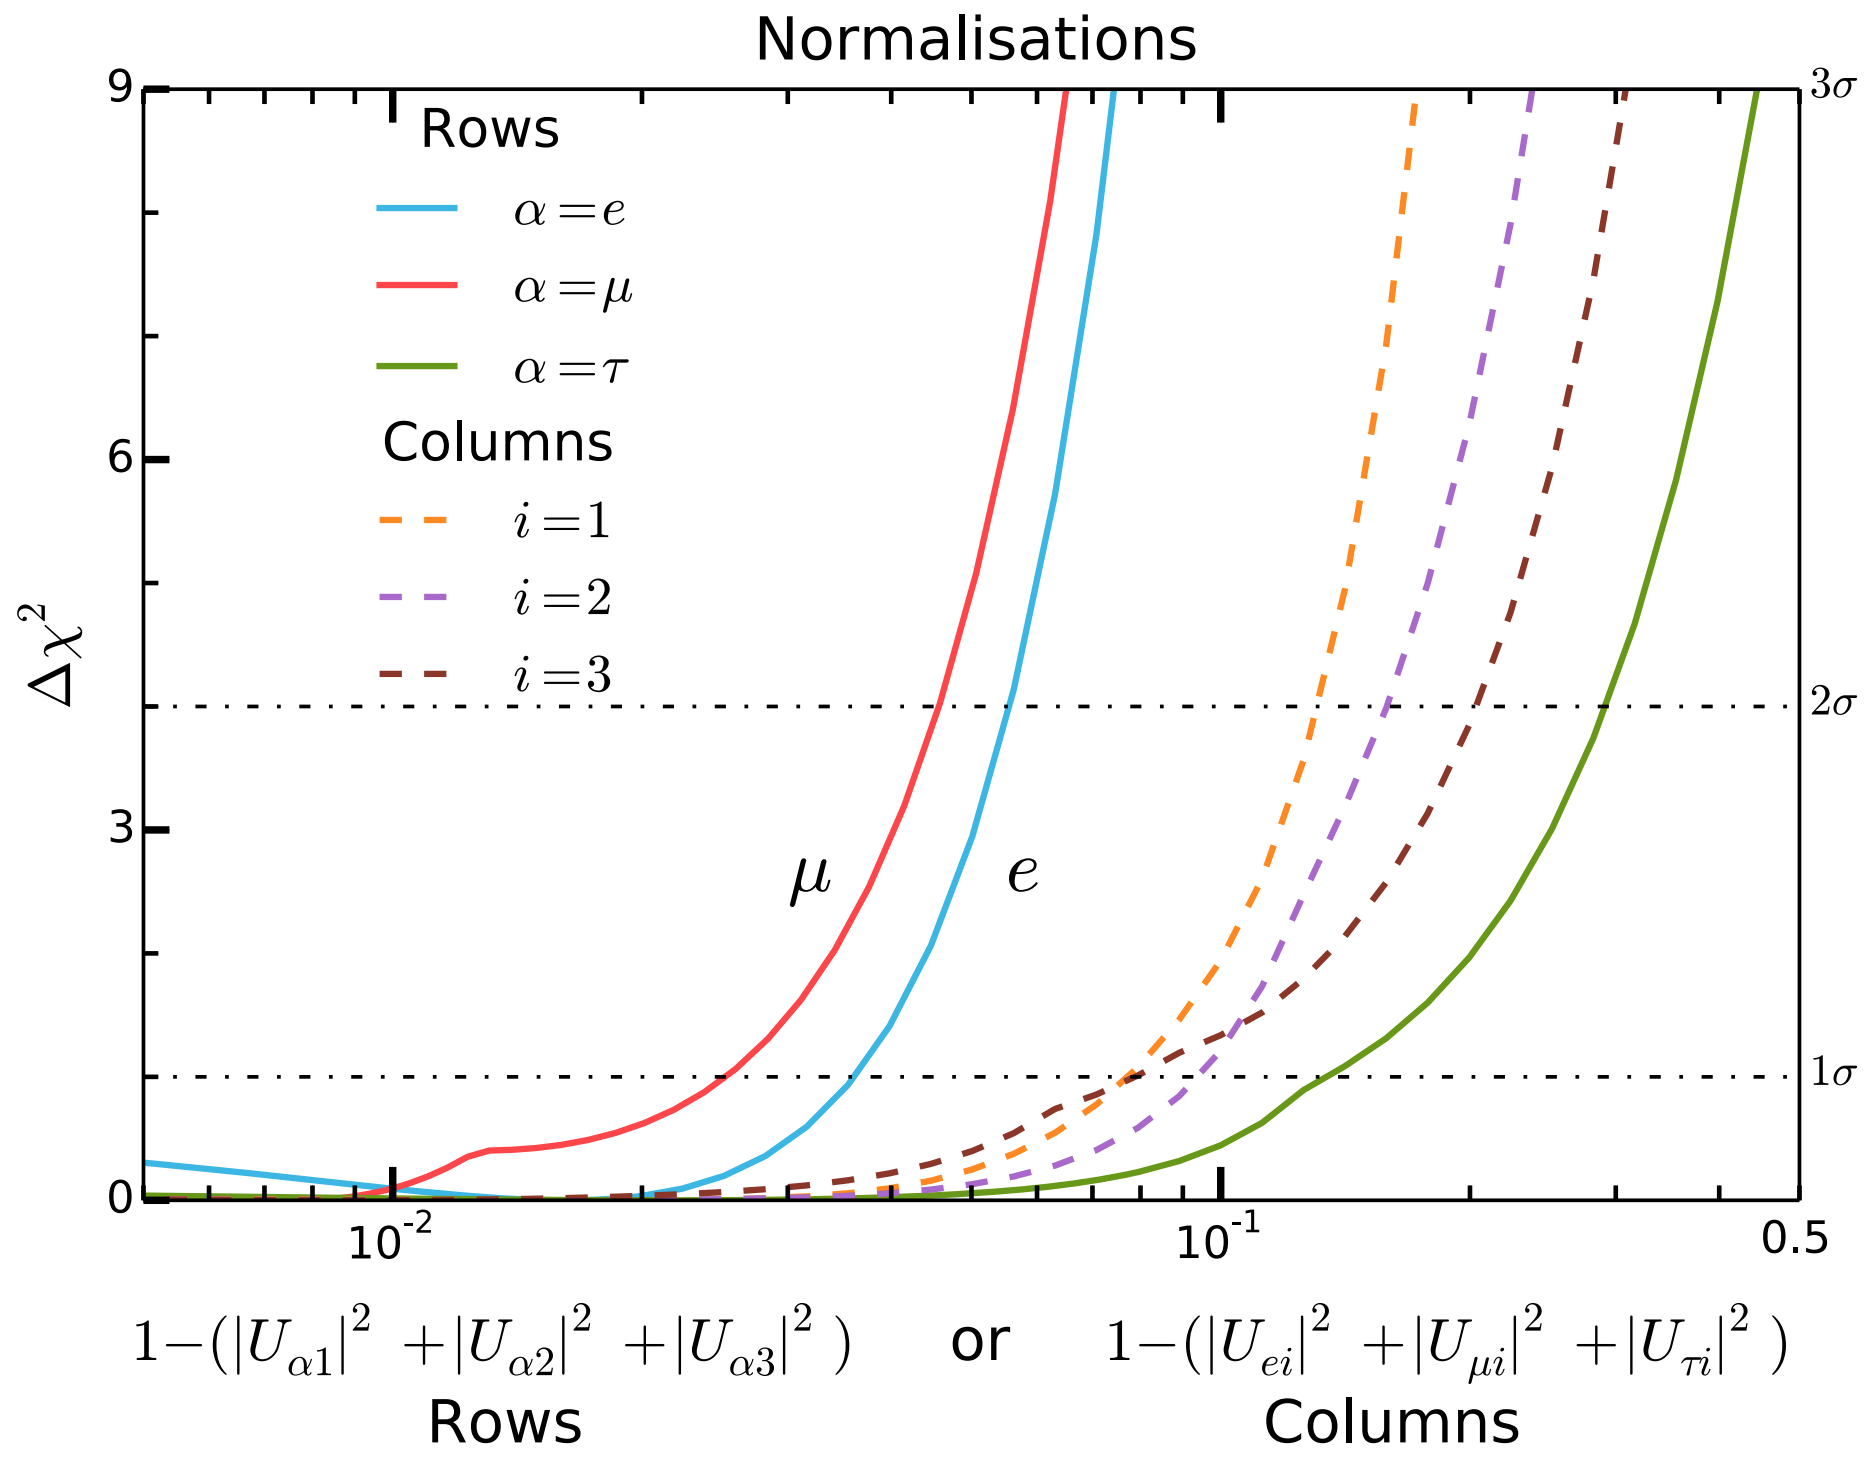
\includegraphics[width=0.7\linewidth]{unitarity_norms.png}%
	\caption[Unitarity normalization tests of the PMNS matrix]{The constraints on unitarity in the rows and columns of the PMNS mixing matrix using Equations~\ref{eqn:unitarity_flavor_test} (solid) and \ref{eqn:unitarity_mass_test} (dotted). A smaller value on the x-axis indicates a tighter constraint on observed unitarity of the 3x3 matrix. Tests involving only muon or electron flavors show significantly tighter constraints than those including the tau flavor. The uncertainties in the tau neutrino mixing elements dominate the total uncertainty in unitarity tests of the PMNS matrix. Image taken from \cite{Parke-Unitarity}}
	\label{fig:unitarity_norms}
\end{figure}

\begin{landscape}
\begin{figure}[!h]%
	\centering
	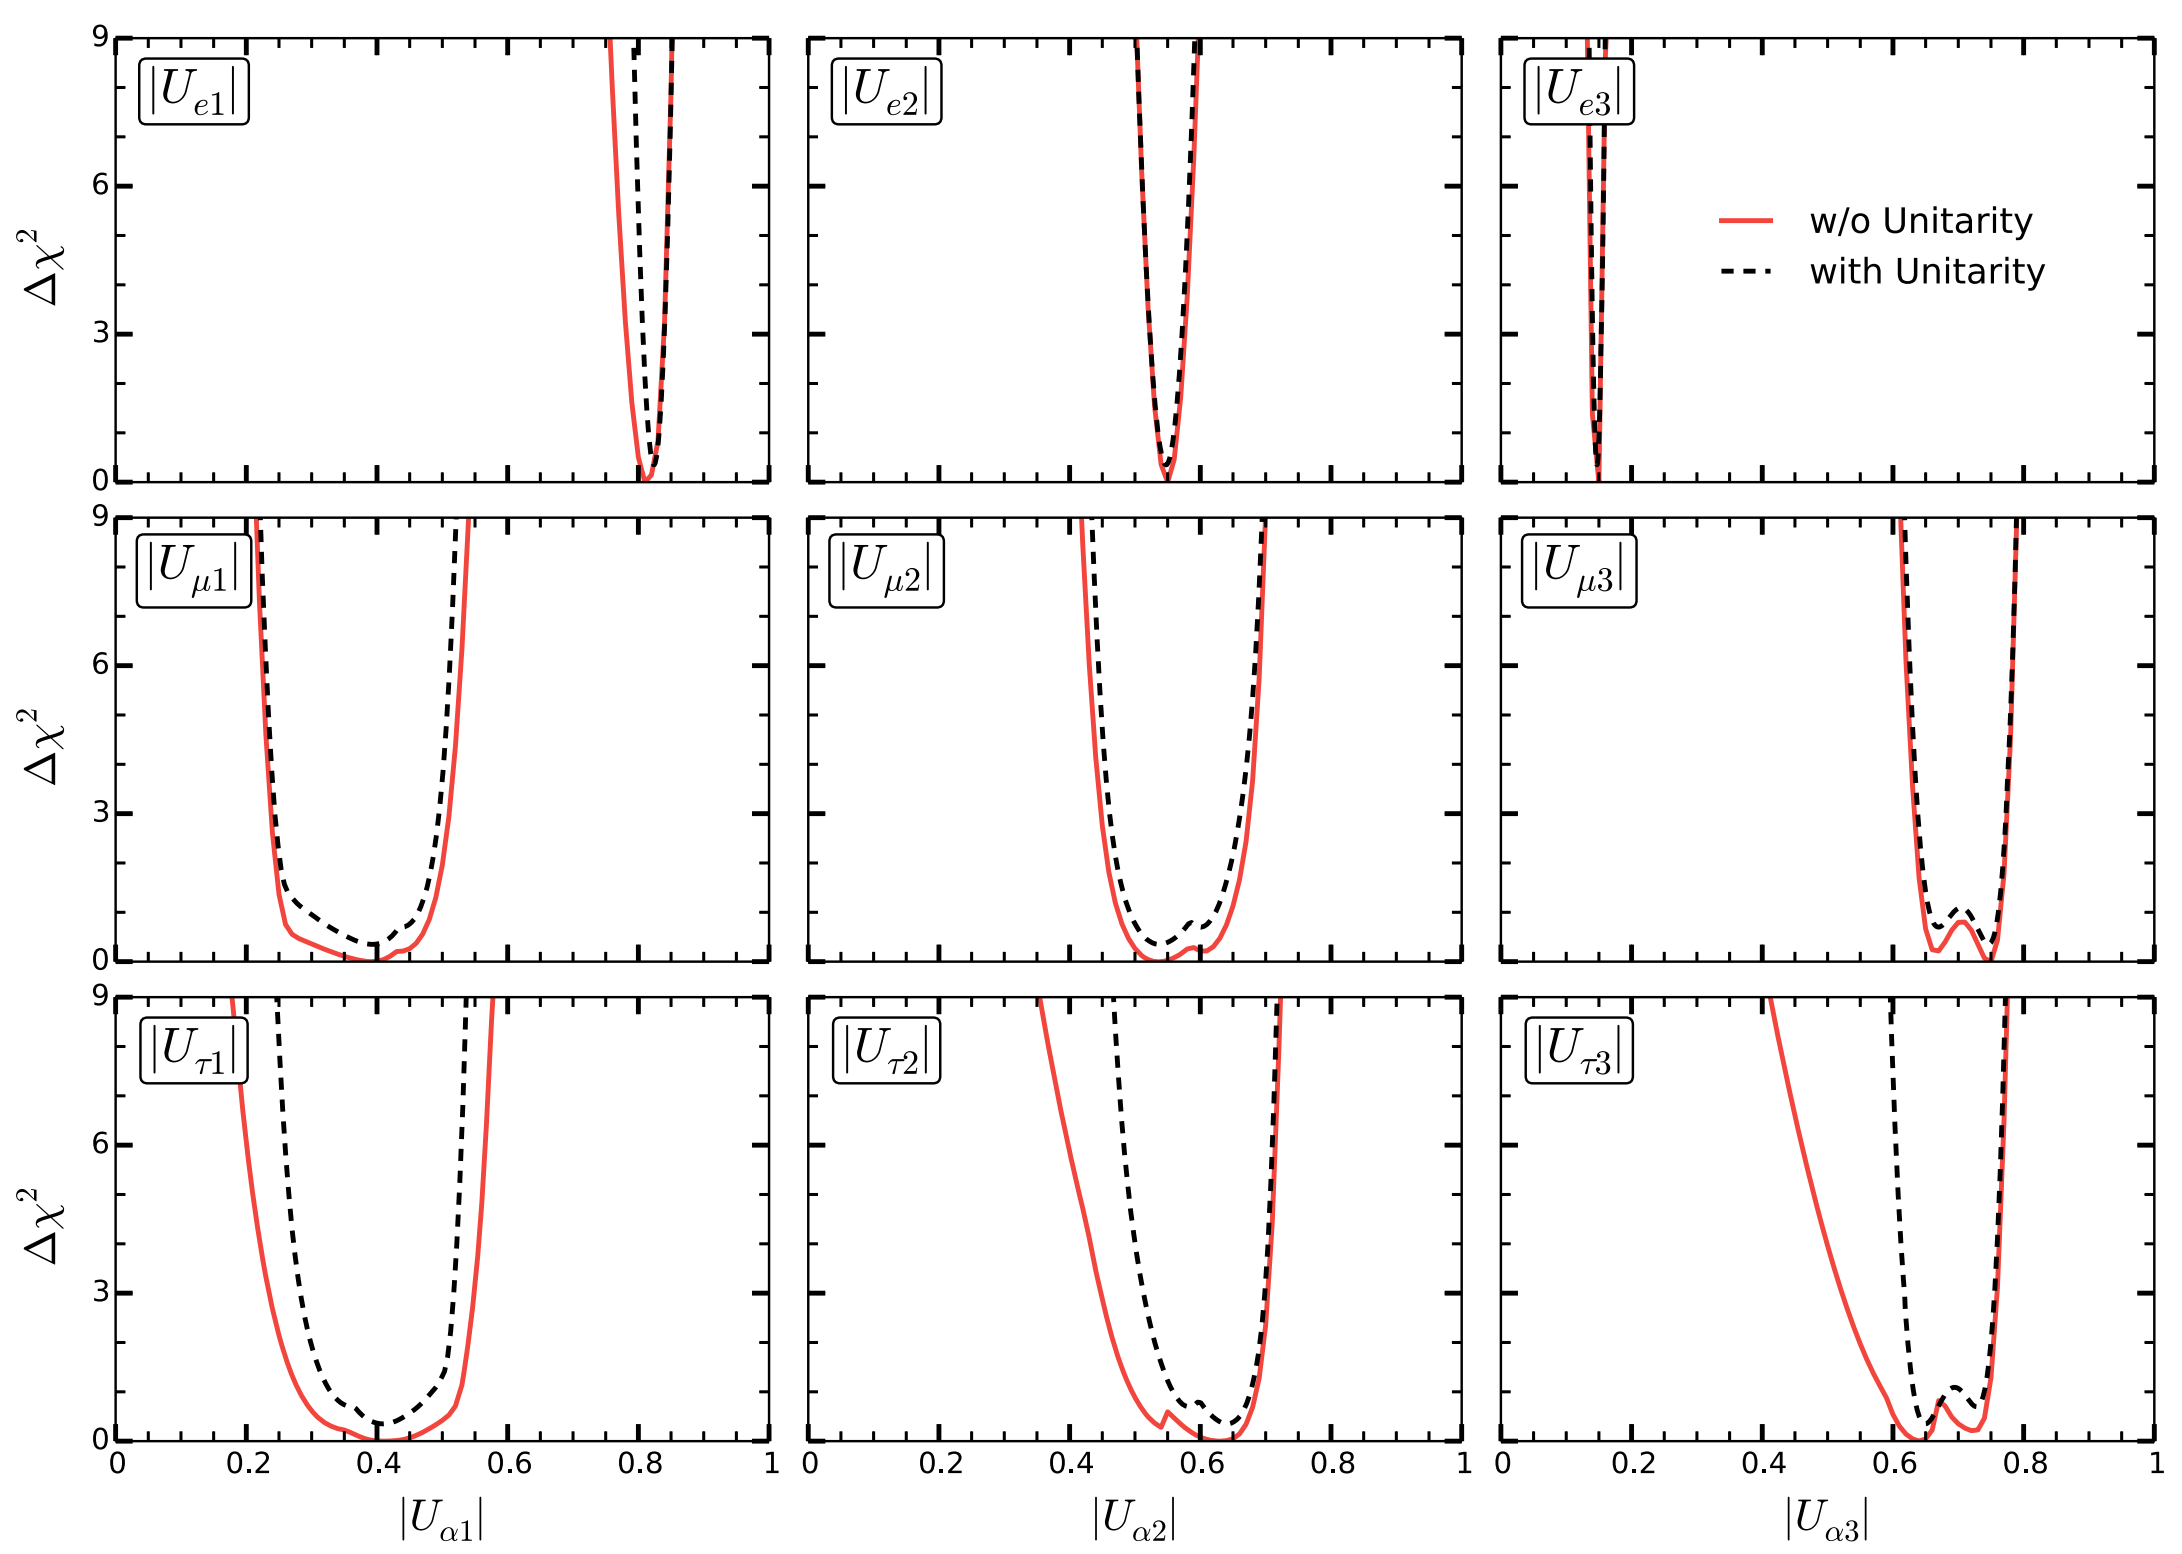
\includegraphics[width=0.8\linewidth]{pmns_unitarity.png}%
	\caption[Constraints on PMNS matrix terms from unitarity]{The constraints from a global fit to neutrino oscillation data\cite{Parke-Unitarity} with an assumption of unitarity (black dotted) or no assumption of unitarity (red solid). The first two rows show little change from the unitarity assumption, indicating strong constraints from direct measurements. The elements of the third row, related to the $\nu_\tau$, show much larger changes, indicating that constraints are obtained from indirect oscillation measurements. }
	\label{fig:pmns_unitarity}
\end{figure}
\end{landscape}

When the individual limits for each element of the 3x3 PMNS matrix are checked in FIgure~\ref{fig:pmns_unitarity}, it is the tau sector that shows the largest uncertainties.
Measurements of $\nu_\tau$ oscillations therefore can provide valuable information on unitarity in the neutrino sector, leading to indirect constaints on sterile neutrino hypotheses.

